\documentclass[a4paper,12pt,oneside]{report} 

% Language setting : English, Vietnamese
\usepackage[utf8]{inputenc}
\usepackage[utf8]{vietnam}
\usepackage[vietnamese=nohyphenation]{hyphsubst}
\usepackage[vietnamese,english]{babel}


% Set page size and margins
\usepackage[a4paper,top=3cm, bottom=3cm, left=3.5cm, right=2cm,marginparwidth=1.75cm]{geometry}

% Useful packages
% Write math equation
\usepackage{amsmath}
\usepackage{float}
% Insert images
\usepackage{graphicx}
\usepackage{fancyhdr}
\usepackage{enumitem}
\usepackage{parskip}
\usepackage{setspace}
\usepackage{tikz}
\usepackage{fancyhdr}	
% \usepackage[square]{natbib}
\usepackage{url}
\usetikzlibrary{calc}
\graphicspath{ {../images/} }


\usepackage[colorlinks=true, allcolors=blue]{hyperref}
\usepackage{tikz}

\title{ASP.NET Souvenir Shop Application}
\author{Nguyen Thanh Phat}

% Header và footer 
\pagestyle{fancy}
\fancyhf{}					% Định dạng cho cả header và footer
\setlength{\headheight}{20.45002pt}
% Header và footer nếu in 1 mặt
\rhead{\fontsize{9}{11} \selectfont Intructor:\\DR. Lam Van Khang}						
\lhead{\fontsize{9}{11} \selectfont Topic:\\ Souvenir Shop App with ASP.NET Microservices \& Flutter}		
\rfoot{\fontsize{9}{11} \selectfont \thepage}														
\lfoot{\fontsize{9}{11} \selectfont Nguyen Thanh Phat - B2005853}		


\begin{document}

% Covers

\begin{titlepage}
    \begin{tikzpicture}[remember picture, overlay]
        %   \draw[line width = 4pt] ($(current page.north west) + (1in,-1in)$) rectangle ($(current page.south east) + (-1in,1in)$);
        \draw [line width=1pt]
        ($ (current page.north west) + (3.0cm,-2.0cm) $)
        rectangle
        ($ (current page.south east) + (-1.5cm,1.5cm) $);
        \draw [line width=3pt]
        ($ (current page.north west) + (3.15cm,-2.15cm) $)
        rectangle
        ($ (current page.south east) + (-1.65cm,1.65cm) $);
    \end{tikzpicture}
    \begin{center}


        % 3 Organization
        % BỘ GIÁO DỤC VÀ ĐÀO TẠO\\
        \textbf{CAN THO UNIVERSITY\\}
        \textbf{COLLEGE OF INFORMATION AND\\ COMMUNICATION TECHNOLOGY\\[1cm]}

        % Logo Cantho University
        
\includegraphics{../images/logo.png}\\[1cm]

        % Project type
        \textbf{PROJECT - SPECIALIZED REPORT \\}
        \textbf{  INFORMATION TECHNOLOGY \\}
        \textbf{(HIGH-QUALITY PROGRAM)\\[1.5cm]}

        % Project title
        % \begin{large}
        %     \textbf{Title\\[0.5cm]}
        % \end{large}
        \textbf{{\Large\ BUILD  SPORT EQUIREMENT\\ ECOMMERCE WEBSITE WITH MEVN STACK}}
        \\[3.5cm]

        % Advisor and student information
        \begin{tabular}{ l l }
            \multicolumn{2}{l}{\textbf{Student:} Nguyen Thanh Phat  } \\
            % Nguyen Thanh Phat        \\
            \multicolumn{2}{l}{\textbf{Student ID:} B2005853}         \\
            \multicolumn{2}{l}{\textbf{Cohort: K46}}                  \\
        \end{tabular}
        \\[4.5cm]

        % Location and datetime
        \textbf{Cantho, 09/2023}

    \end{center}

\end{titlepage}


\begin{titlepage}

    \begin{center}

        % 3 dòng chữ về tổ chức
        BỘ GIÁO DỤC VÀ ĐÀO TẠO\\
        \textbf{TRƯỜNG ĐẠI HỌC CẦN THƠ\\}
        \textbf{TRƯỜNG CÔNG NGHỆ THÔNG TIN VÀ TRUYỀN THÔNG\\[1cm]}

        % Logo Đại học Cần Thơ
        
\includegraphics{logo.png}\\[1cm]

        % Luận văn
        \textbf{BÁO CÁO NIÊN LUẬN CHUYÊN NGÀNH\\}
        \textbf{NGÀNH CÔNG NGHỆ THÔNG TIN\\[2cm]}

        % Tên đề tài
        \begin{large}
            \textbf{Đề tài\\[0.5cm]}
        \end{large}
        \textbf{{\LARGE XÂY DỰNG DỤNG THƯƠNG MẠI \\ SỬ DỤNG FLUTTER VÀ ASP.NET API}}
        \\[3.5cm]

        % Tên sinh viên thực hiện và người hướng dẫn 
        \begin{tabular}{ l c l l }
            \textbf{Giảng viên hướng dẫn:} & \hspace{2cm} & \multicolumn{2}{l}{\textbf{Sinh viên thực hiện:}}   \\
            TS. Lâm Văn Khang              &              & Nguyễn Thanh Phát                                 &
            B2005853                                                                                            \\
                                           &              & \multicolumn{2}{l}{\textbf{Khóa:} 46}
        \end{tabular}
        \\[4cm]

        % Địa điểm, ngày tháng 
        \textbf{Cần Thơ, 09/2023}

    \end{center}

\end{titlepage}

% Table of Content
\tableofcontents
\listoffigures
\listoftables


% English Abtract
\begin{abstract}
    This project is aimed at creating an online marketplace for sports equipment, offering users a seamless and intuitive shopping experience. The website will be developed using the MEVN stack (MongoDB, Express.js, Vue.js, Node.js), supplemented with Bootstrap for responsive design, and TypeScript for static typing, enhancing code quality and understandability.

    The development process will adhere to the principles of the Minimum Viable Product (MVP) approach, resulting in a compact, single-tiered website. This approach ensures the system is scalable, maintainable, and provides a rich, user-friendly interface.
    
    The project’s scope is concentrated on fulfilling the essential features of an e-commerce website, including product listing, shopping cart functionality, order processing, user authentication, wishlist management, and product reviews.
    
    The anticipated outcomes of this project include a deeper comprehension of full-stack web development using the MEVN stack, understanding the MVP approach, and gaining insights into the operational aspects of an e-commerce website. This project serves as a practical application of these technologies and concepts, demonstrating their effectiveness in a real-world scenario.
\end{abstract}

% Vietnamese Abstract
\selectlanguage{vietnamese}
\begin{abstract}
    Dự án này nhằm mục đích tạo ra một thị trường trực tuyến cho thiết bị thể thao, mang đến cho người dùng trải nghiệm mua sắm liền mạch và trực quan. Trang web sẽ được phát triển bằng MEVN stack (MongoDB, Express.js, Vue.js, Node.js), được bổ sung Bootstrap cho thiết kế đáp ứng và TypeScript cho kiểu tĩnh, nâng cao chất lượng và khả năng hiểu của mã.

    Quy trình phát triển sẽ tuân theo các nguyên tắc của phương pháp Sản phẩm tối thiểu khả thi (MVP), dẫn đến một trang web nhỏ gọn, một tầng. Phương pháp này đảm bảo hệ thống có khả năng mở rộng, dễ bảo trì và cung cấp giao diện người dùng phong phú, thân thiện.

    Phạm vi của dự án tập trung vào việc đáp ứng các tính năng thiết yếu của một trang web thương mại điện tử, bao gồm liệt kê sản phẩm, chức năng giỏ hàng, xử lý đơn hàng, xác thực người dùng, quản lý danh sách mong muốn và đánh giá sản phẩm.

    Các kết quả dự kiến của dự án bao gồm sự hiểu biết sâu sắc hơn về phát triển web full-stack bằng MEVN stack, hiểu được phương pháp MVP và thu được thông tin chi tiết về các khía cạnh hoạt động của trang web thương mại điện tử. Dự án này đóng vai trò là ứng dụng thực tế của các công nghệ và khái niệm này, thể hiện hiệu quả của chúng trong một tình huống thực tế.\end{abstract}
\selectlanguage{english}
\pagenumbering{roman}

\clearpage
\pagenumbering{arabic}
\chapter{Introduction}
% What is the motivation for your research?
% What problem are you trying to solve with your application?
% What are your research questions?
% What are the main contributions of your thesis?
\section{Background}
The rise of information technology has significantly impacted business operations, with software applications becoming integral to sales operations. However, choosing the right software and platform can be challenging, especially for small and medium-sized enterprises (SMEs).

Traditionally, many businesses have used monolithic architecture, a unified and self-contained model. While this model is convenient in the early stages of a project, it can become complex and hard to manage as the application grows.

To address these challenges, businesses are now turning to the MEVN stack (MongoDB, Express.js, Vue.js, Node.js). This stack allows for a scalable and maintainable system, providing a rich, user-friendly interface.

For instance, a sport equipment shop website can be developed using the MEVN stack. By breaking down the application into smaller parts, it's easier to scale services based on demand and deploy updates more frequently without disrupting the entire system.

Sport equipment shop websites can use the MEVN stack to manage products, inventory, orders, and payments, making it easier to add new features, scale as needed, and ensure system reliability.
\section{Problem statement}
% The traditional monolithic architecture, while convenient early on, becomes less efficient as the application grows in size. To address these challenges, the e-shop needs to adopt microservices architecture.
\textbf{Challenge}: E-commerce enterprises, particularly SMEs, face the challenge of selecting scalable software solutions that can accommodate their growth trajectory. While monolithic architectures initially offer simplicity in code management and deployment, they become increasingly complex and unwieldy as applications expand.

\textbf{Solution}: To address these challenges, there is a need for a new approach: the MEVN stack (MongoDB, Express.js, Vue.js, Node.js). This stack allows for a scalable and maintainable system, providing a rich, user-friendly interface.

\textbf{Objective}: The objective of this project is to implement a new sport equipment shop website using the MEVN stack from the ground up. The website will have minimal features due to the project's short deadline.

\textbf{Aim:} By adopting the MEVN stack from the start, the sport equipment shop website aims to develop and deploy new features more easily, scale as needed, and improve the overall reliability of the system.

% What are your research questions?
\section{Research Objectives}
The primary aim of this project is to design and implement a microservices-based e-commerce application for a souvenir e-shop, along with a front-end application using Flutter. The specific objectives are as follows:
\begin{itemize}
    \item[-] \textbf{Literature Review:} Conduct a comprehensive review of existing literature on the MEVN stack, its benefits, challenges, and best practices. This will provide a theoretical foundation for the project.
    \item[-] \textbf{Design:} Design a MEVN-based e-commerce application model. The design should consider factors such as scalability, fault tolerance, and ease of adding new features. In parallel, design a front-end application using Vue.js.
    \item[-] \textbf{Development:} Develop a minimum viable product (MVP) of an e-commerce application for a sport equipment shop website using the proposed model. The MVP will include key features such as product management, inventory management, order processing, and payment processing.
    \item[-] \textbf{Documentation:} Document the entire process, including the design decisions made, challenges encountered, solutions implemented, and lessons learned. This will serve as a valuable resource for future projects of similar nature.
\end{itemize}
% What are the main contributions of your thesis?
\section{Research Scope}
The focus of this research is on the design and implementation of a MEVN-based e-commerce application for a sport equipment shop website.
The specific areas covered in this research include:
\begin{itemize}
    \item[-] \textbf{MEVN Stack:} The research will delve into the principles and practices of the MEVN stack. It will explore how to design and implement an e-commerce application using this stack.
    \item[-] \textbf{Front-end Development with Vue.js: } he research will also cover the design and implementation of a front-end application using Vue.js.
    \item[-] \textbf{Key Features: } The research will focus on implementing key features for an e-commerce application, such as product management, inventory management, order processing, and payment processing.
    \item[-] \textbf{Evaluation:} The research will include an evaluation of the implemented system in terms of functionality, performance, scalability, and reliability.
\end{itemize}

Please note that while the research aims to cover these areas, it is limited by the project's short time. Therefore, the e-shop application developed as part of this project will be a minimum viable product (MVP) with basic features.
\section{Solution approach}
The approach to solving the problem at hand involves several steps, each designed to ensure the successful implementation of a microservices-based e-commerce application for a souvenir e-shop, along with a front-end application using Flutter. The steps are as follows:
\begin{enumerate}
    \item[-] \textbf{Literature Review:} The first step involves conducting a comprehensive review of existing literature on the MEVN stack. This will provide a theoretical foundation for the project and inform the design and implementation stages.
    \item[-] \textbf{Design:} The next step is to design the MEVN-based e-commerce application model. The design will take into account factors such as scalability, fault tolerance, and ease of adding new features.
    \item[-] \textbf{Development:} Once the design is complete, the development of the minimum viable product (MVP) begins. This involves coding the back-end services and front-end application, and setting up the necessary databases and interfaces.
    \item[-] \textbf{Testing: :} After the MVP is developed, it will be thoroughly tested to ensure it functions as expected. This includes unit testing, integration testing, and system testing.
    \item[-] \textbf{Evaluation:} The MVP will then be evaluated in terms of its functionality, performance, scalability, and reliability. Feedback from this evaluation will be used to identify areas for improvement.
\end{enumerate}

\section{Report structure}
% Trong giai đoạn luận văn đề tài  đã thực hiện được một số công việc liên quan sẽ trình bày trong báo cáo như sau:
% % \setlist[enumerate]{leftmargin=*}
\begin{enumerate}[label=\bfseries Chapter \arabic*.,leftmargin=*]
    \item \textbf{Introduction:} This chapter provides a general overview of the topic, its potential, and practical applications in the future. It introduces the concept of a MEVN-based e-commerce application for a sport equipment shop website.
    \item \textbf{Literature review} This section provides a summary of relevant research on the topic and the foundational knowledge necessary to develop an e-commerce application using the MEVN stack.
          % \item \textbf{Methods} This section provides 
    \item \textbf{System design and implementation} This section presents the approach to the problem. It discusses the details of the implementation approach, including the tools used.
    \item \textbf{Testing and evaluation.}  This chapter presents the testing plan and management, testing scenarios for the main functions of the system.
    \item \textbf{Conclusion} This section presents the results achieved, the remaining limitations, and the system’s further development.
\end{enumerate}




\chapter{Literature reiview}
The aim of this literature review is to provide a comprehensive understanding of the key concepts and technologies that underpin this project. These include the MEVN stack and front-end development using Vue.js. This review will serve as the theoretical foundation for the design and implementation of a MEVN-based e-commerce application for a sport equipment shop website.

In the next section, we will delve deeper into the MEVN stack, starting with its definition and core principles.
\section{Microservices Architecture}
\subsection{Overview of Microservices Architecture}
Microservices architecture is a design approach where an application is built as a collection of small services. Each of these services runs in its own process and communicates with others using lightweight mechanisms, often an HTTP resource API. These services are built around business capabilities and are independently deployable by fully automated deployment machinery.
\begin{figure}[H]
    \centering
    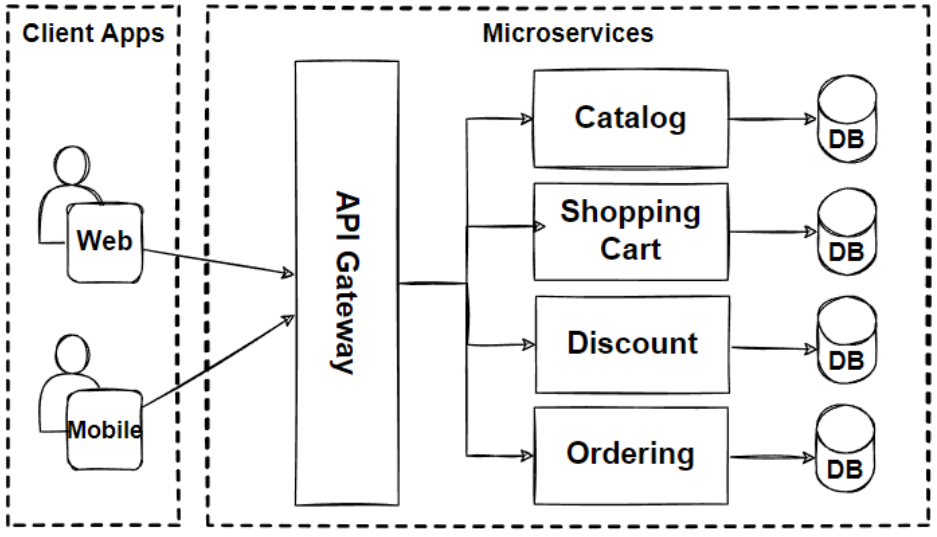
\includegraphics[width=.64\linewidth]{../images/micoservices_visualization.png}
    \caption{Microservices}\label{Fig:NN}
\end{figure}

For instance, consider an e-commerce application. In a monolithic architecture, all functionalities like user management, product catalog, order processing, and payment system would be in a single codebase. In contrast, in a microservices architecture, each of these functionalities would be a separate service with its own database and business logic.

\subsection{Benefits of Microservices:}
The benefits of using microservices architecture in e-commerce applications are numerous. They include improved scalability as each service can be scaled independently based on demand, increased resilience as the failure of a single service does not affect the entire system, and enhanced agility and speed in bringing new features to market.

\textbf{Amazon} is a prime example of the benefits of microservices. Originally, Amazon had a monolithic architecture, but as their services expanded, they moved to a microservices architecture. This allowed them to scale individual services based on demand. For example, during a sale, the order processing service could be scaled up without affecting other services.

\subsection{Challenges of Microservices:}

Despite its benefits, microservices architecture presents several challenges:
\begin{itemize}
    \item[-] \textbf{Complexity:} Managing multiple services can be complex, requiring sophisticated coordination and orchestration.
    \item[-] \textbf{Distributed Data Management:} Handling distributed data across services can be difficult and requires careful consistency management.
    \item[-] \textbf{Communication Overhead:} Implementing communication between services can introduce additional latency and resource usage.
\end{itemize}

\textbf{Netflix} faced challenges with microservices when they first transitioned from a monolithic architecture. They had to deal with complexities in managing multiple services and ensuring data consistency across services. They also faced challenges in implementing communication between services.

\section{Microservices in ASP.NET}
In this project, a new souvenir e-shop will be implemented using a microservices architecture from the ground up with ASP.NET. Each feature such as product management, inventory management, order processing, and payment processing will be implemented as a separate microservice running in its own Docker container.
\subsection{ASP.NET and Microservices}
ASP.NET is a robust framework for .NET that simplifies the creation of APIs, which form the backbone of microservices. It provides built-in support for Docker containers, which are lightweight and can be easily managed, making them ideal for deploying microservices.

ASP.NET offers high performance, which is critical in a microservices architecture where each service should be highly responsive. The high throughput of .NET surpasses many popular frameworks, making it an excellent choice for building efficient microservices.
\subsection{Communication Between Services}
In a microservices architecture built with ASP.NET, secure communication between services is crucial. Technologies like HTTPS provide secure communication over a computer network, while RabbitMQ with MassTransit in ASP.NET offers a reliable and efficient message broker system, which is essential for communication between microservices.

\subsection{Docker and .NET Tools}
Docker has become a standard in the container industry due to its ability to encapsulate microservices in containers, enhancing their isolation, portability, and scalability. .NET is built to work seamlessly with Docker, allowing developers to focus on building their microservices without worrying about compatibility issues.

The Visual Studio family of products offers comprehensive tools for developing ASP.NET applications with Docker support on Windows.
These tools simplify the process of configuring applications for Docker and allow developers to step through their code line-by-line as it runs in a Docker container.
\section{Introduction to Flutter and Clean Architecture}
\subsection{Flutter}
Flutter is an open-source UI software development kit created by Google. It is used to develop cross platform applications for Android, iOS, Linux, Mac, Windows, Google Fuchsia, and the web from a single codebase. Key features of Flutter include its fast development cycle, expressive and flexible UI, and native performance.
\subsection{Clean Architecture}
Clean Architecture is a software design philosophy that separates software into layers with ‘stable dependencies’. This architecture promotes the separation of concerns, making the system easier to manage and maintain. It is important because it makes the system more flexible, maintainable, and scalable.
\begin{figure}[H]
    \centering
    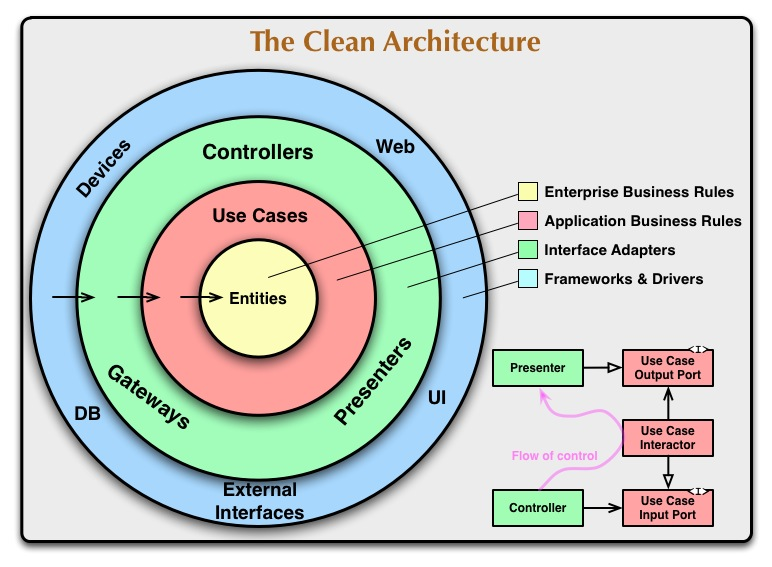
\includegraphics[width=.84\linewidth]{../images/clean-architecture-by-robert-c-martin.jpg}
    \caption{Clean architecture by Robert C. Martin \cite{unclebob2023}}\label{Fig:CABRMARTIN}
\end{figure}
\subsection{Applying Clean Architecture in Flutter}
Clean Architecture can be applied in Flutter by separating the application into three layers: Presentation, Domain, and Data. The Presentation layer handles the UI and user interactions. The Domain layer contains business logic and use cases. The Data layer manages data from various sources like network requests and databases.
\begin{figure}[H]
    \begin{minipage}{0.60\textwidth}
        \centering
        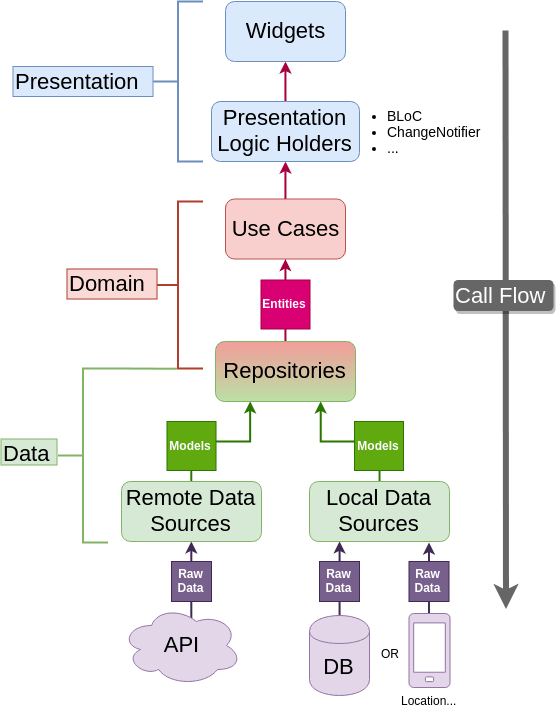
\includegraphics[width=1\linewidth]{../images/Clean-Architecture-Flutter-Diagram.png}
        \caption{Clean Architecture Diagram by Reso Coder\cite{resocoder2019course1}}\label{Fig:CADRESOCODER}
    \end{minipage}\hfill
    \begin {minipage}{0.38\textwidth}
    \centering
    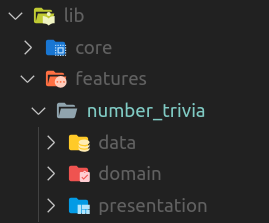
\includegraphics[width=\linewidth]{../images/number_trivia-feature-folder-structure.png}
    \caption{Example of structure in Flutter project}\label{Fig:example-flutter-ca-folder}
    \end{minipage}
\end{figure}
\section{Applications of Flutter and Clean Architecture}
\subsection{Accelerated MVP Development with Flutter}
Flutter's ability to deliver high-performance applications on Android and iOS from a single codebase makes it an excellent choice for rapid MVP development. Its rich set of widgets and reactive framework allow for a fast development cycle, enabling developers to quickly implement key features and bring the product to market.
\subsection{Case Studies of Flutter and Clean Architecture}
There are several case studies of applications developed using both Flutter and Clean Architecture. These applications demonstrate how Clean Architecture can enhance the maintainability and scalability of Flutter applications, even when under the constraints of rapid MVP development.

Flutter has been used in various real-world applications due to its ability to deliver high-performance applications on Android and iOS from a single codebase. Some examples include the Alibaba e-commerce app, the Toyota: Improving Infotainment Systems app, and Google Ads.

\begin{figure}[H]
    \begin{minipage}{0.48\textwidth}
        \centering
        
\includegraphics[width=1\linewidth]{../images/alibaba-commerce.png}
        \caption{Alibaba Group: Ecommerce}\label{Fig:AGEAPP}
    \end{minipage}\hfill
    \begin {minipage}{0.48\textwidth}
    \centering
    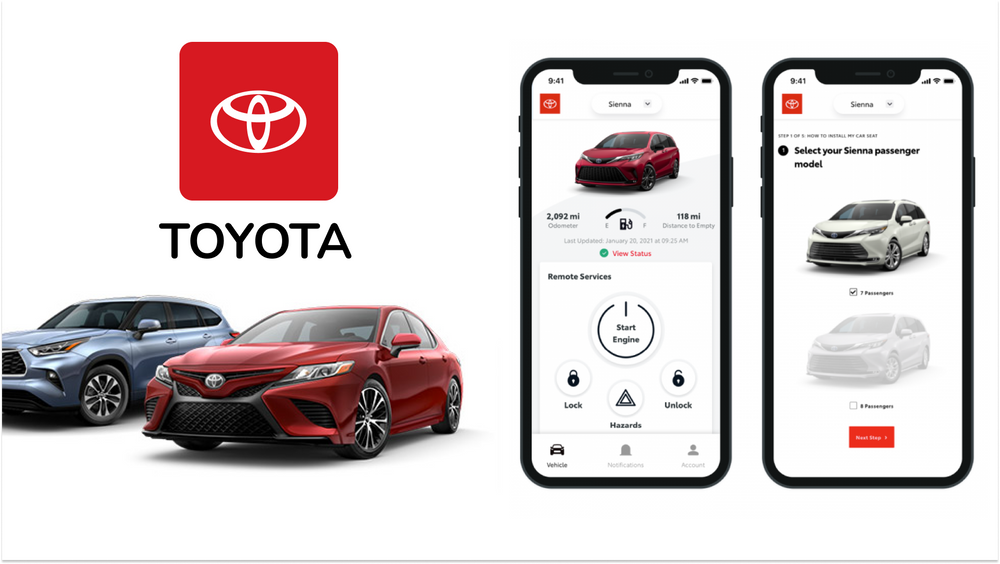
\includegraphics[width=\linewidth]{../images/TOYOTA-1.png}
    \caption{Toyota: Improving Infotainment Systems}\label{Fig:TIISAPP}
    \end{minipage}
\end{figure}
\subsection{Impact of Flutter and Clean Architecture}
The use of Flutter along with Clean Architecture has been shown to improve the development process by making it easier to manage codebases, implement new features, and fix bugs. It also enhances the performance of applications by ensuring they run smoothly on different platforms.

\section{Microservices, Flutter, and E-commerce}

\subsection{Application of Microservices and Flutter in E-commerce}
Microservices architecture and Flutter can be effectively applied in the context of e-commerce. Microservices allow for the separation of functionalities into independent services such as user authentication, product catalog, order management, and payment processing1. Flutter, with its fast development cycle and expressive UI, can be used to build the frontend of the e-commerce application.

\subsection{Benefits and Challenges}
The benefits of using these technologies in e-commerce include improved scalability, faster deployment times, better fault isolation, and more flexibility in implementing new features. However, challenges may include increased dependency on technology, large costs involved especially for small businesses, risk of job cuts due to automation, security risks related to data and fraud, and dealing with issues like shopping cart abandonment and maintaining customer loyalty.

\subsection{Case Studies}
Several e-commerce giants like eBay, Etsy, Gilt and Zalando have transformed their infrastructures into microservice architectures to create flexible, global systems. The combination of these technologies holds promise for efficient and scalable e-commerce application development.

% \chapter{Methods}
% \input{chapters/chapter-3-methods.tex}

\chapter{System design and implementation}
\section{Section 1}

\chapter{Testing and evaluation.}
\section{Section 1}

\chapter{Conclusion}
\section{Section 1}

\bibliography{references}{}
\bibliographystyle{plain}


\end{document}